%
% File acl2010.tex
%
% Contact  jshin@csie.ncnu.edu.tw or pkoehn@inf.ed.ac.uk
%%
%% Based on the style files for ACL-IJCNLP-2009, which were, in turn,
%% based on the style files for EACL-2009 and IJCNLP-2008...

%% Based on the style files for EACL 2006 by 
%%e.agirre@ehu.es or Sergi.Balari@uab.es
%% and that of ACL 08 by Joakim Nivre and Noah Smith

\documentclass[11pt]{article}
\usepackage{acl2010}
\usepackage{times}
\usepackage{url}
\usepackage{latexsym}
\usepackage{graphicx}
%\setlength\titlebox{6.5cm}    % You can expand the title box if you
% really have to
\usepackage{color}

\definecolor{red}{rgb}{1,0,0}

\newcommand{\mnote}[1]{\marginpar{%
  \vskip-\baselineskip
  \raggedright\footnotesize
  \itshape\hrule\smallskip\tiny{#1}\par\smallskip\hrule}}  

\newcommand{\mtodo}[1]{\mnote{\textcolor{red}{#1}}}

\title{Bilingual Lexicon Induction for Less Commonly Used Languages}

%\author{Blah\\
%  JHU\\
%  Madltimore, MD.\\
%  {\tt blah@jhu.edu}  \And
%  Blah\\
%  JHU\\
%  Baltimore, MD.\\
%  {\tt  blah@jhu.edu}}

\date{}

\begin{document}
\maketitle
\begin{abstract}
\end{abstract}

\section{Introduction} \label{sect:intro}

\section{Inducing Bilingual Lexicons} \label{sect:lexinduct}

Cues and similarity metrics:
\begin{itemize}
\setlength{\parskip}{0pt}
  \item Context (including contextual NEs), using dependency contexts for the resources rich side (i.e. English).
  \item Time
  \item Topics (i.e. wiki categories)
  \item Edit distance
\end{itemize}

\noindent Combination strategies:
\begin{itemize}
\setlength{\parskip}{0pt}
  \item cue scores as classification features: use seed dictionaries for supervised data.
  \item rank aggregation
\end{itemize}

\noindent Evaluation:  tokens for inducing translations.  Evaluation metrics: why precision at top-k?

\section{Experimental Evaluation} \label{sect:exp}

\subsection{Data and Other Resources}

Describe the data:
\begin{itemize}
  \item Wiki
  \item News
\end{itemize}

\noindent Describe the resources:
\begin{itemize}
  \item Dictionaries: generally, noisy
  \item Parallel data: some languages may have small amounts of parallel data
\end{itemize}

\subsection{Quality of Available Resources}

Parallel data experiments:
\begin{itemize}
  \item Moses lexical tables vs. monolingual cues (e.g., Fig. \ref{fig:parvsmono}).
  \item Use Moses lexical tables as seed dictionaries.
\end{itemize}

\begin{figure}
\begin{center}
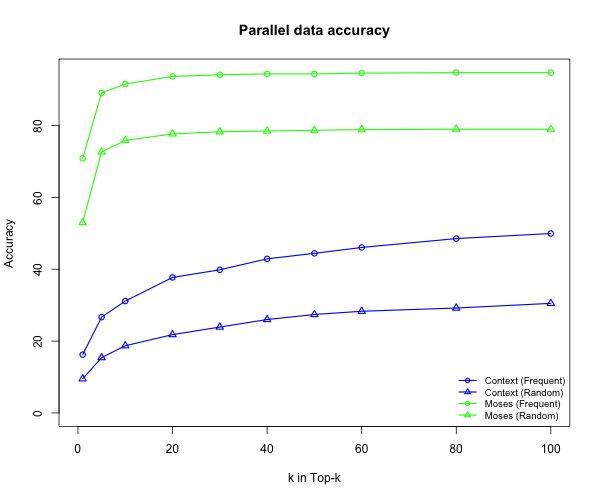
\includegraphics[width=3in]{figures/mostfreqrand.png}
\caption{Bilingual lexicons from Moses lexical tables vs. using contextual cues.} \label{fig:parvsmono}
\end{center}
\end{figure}

\subsection{Quality of Individual Cues} 

Performance of individual cues per language.

\subsection{Combination strategies}

Classification and rank aggregation.

\section{Related Work} \label{sect:relwork}

\begin{itemize}
\setlength{\parskip}{0pt}
  \item Context: \cite{Rapp:1995,Rapp:1999,Fung:1998}
  \item Time: \cite{Schafer:2002,Klementiev:2006b}
  \item Topics: \cite{Mimno:2009,Boyd-Graber:2009}
  \item Multiple: \cite{Schafer:2002,Koehn:2000,Haghighi:2008}
  \item Dependecies: \cite{Garera:2009}
  \item Bridge languages: \cite{Mann:2001}
  \item Combination Strategies: \cite{Koehn:2000,Klementiev:2006b,Klementiev:2008a}
  \item Mechanical Turk: Our NAACL workshop paper.
  \item Other: \cite{Monz:2005}
\end{itemize}

\section{Conclusions and Future Work} \label{sect:conclusions}

Using cues for MT.

\section*{Acknowledgments}

\bibliographystyle{acl}
\bibliography{AlexBib}

\end{document}
